\documentclass[12pt,titlepage]{article}
\usepackage[margin=1.25in]{geometry}
\usepackage{graphicx,amsmath,blindtext,minted}

%% Variables definition
\newcommand{\vSubject}{Data Structure and Algorithm Practicum}
\newcommand{\vSubtitle}{Searching}
\newcommand{\vName}{Dicha Zelianivan Arkana}
\newcommand{\vNIM}{2241720002}
\newcommand{\vClass}{1i}
\newcommand{\vDepartment}{Information Technology}
\newcommand{\vStudyProgram}{D4 Informatics Engineering}

%% [START] Tikz related stuff
\usepackage{tikz}
\usetikzlibrary{svg.path,calc,shapes.geometric,shapes.misc}
\tikzstyle{terminator} = [rectangle, draw, text centered, rounded corners = 1em, minimum height=2em]
\tikzstyle{preparation} = [chamfered rectangle, chamfered rectangle sep=0.75em, draw, text centered, minimum height = 2em]
\tikzstyle{process} = [rectangle, draw, text centered, minimum height=2em]
\tikzstyle{decision} = [diamond, aspect=2, draw, text centered, minimum height=2em]
\tikzstyle{data}=[trapezium, draw, text centered, trapezium left angle=60, trapezium right angle=120, minimum height=2em]
\tikzstyle{connector} = [line width=0.25mm,->]
%% [END] Tikz related stuff

%% [START] Fancy header related stuff
\usepackage{fancyhdr}
\pagestyle{fancy}
\setlength{\headheight}{15pt} % compensate fancyhdr style
\fancyhead{}
\fancyfoot{}
\fancyfoot[L]{\thepage}
\fancyfoot[R]{\textit{\vSubject - \vSubtitle}}
\renewcommand{\footrulewidth}{0.4pt}% default is 0pt, overline for footer
%% [END] Fancy header related stuff

%% [START] Custom tabular command related stuff
\usepackage{tabularx}
\newcommand{\details}[2]{
    #1 & #2  \\
}
%% [END] Custom tabular command related stuff

%% [START] Figure related stuff
\newcommand{\image}[3][1]{
    \begin{figure}[h]
        \centering
        \includegraphics[#1]{#2}
        \caption{#3}
        \label{#3}
    \end{figure}
}
%% [END] Figure related stuff

\begin{document}
\begin{titlepage}
    \centering
    \vfill
    {\bfseries\LARGE
        \vSubject\\
        \vskip0.25cm
        \vSubtitle
    }
    \vfill
    
\includegraphics[width=6cm]{images/polinema-logo.png}
    \vfill
    {
        \textbf{Name}\\
        \vName\\
        \vskip0.5cm
        \textbf{NIM}\\
        \vNIM\\
        \vskip0.5cm
        \textbf{Class}\\
        \vClass\\
        \vskip0.5cm
        \textbf{Department}\\
        \vDepartment\\
        \vskip0.5cm
        \textbf{Study Program}\\
        \vStudyProgram
    }
\end{titlepage}

\section{Sequential Search Method}
\subsection{Questions}
\begin{enumerate}
    \item {
        What is the difference of method \texttt{displayData()} and \texttt{displayPosition()} in \texttt{StudentSearch} class?

        The former shows the entire data of the student while the latter only shows the position of the student.
    }
    \item {
        What is the function of break in this following program code?

        \begin{minted}[autogobble,fontsize=\small]{java}
            if (listStudents[i].nim == search) {
                position = i;
                break;
            }
        \end{minted}

        It's used to break the loop when we found the matching student's nim.
    }
    \item {
        If inserted NIM data is not sorted from smallest to biggest value, will the program encounter an error? 
        Is the result still correct? Why is that?

        Because linear search doesn't depend on the sorting, it won't throw an error. It works by checking each item from start to finish.
    }
\end{enumerate}

\section{Binary Search Method}
\subsection{Questions}
\begin{enumerate}
    \item {
        Show the program code in which runs the divide process

        \begin{minted}[autogobble,fontsize=\small]{java}
            if (search == listStudents[mid].nim) {
                return mid;
            } else if (listStudents[mid].nim > search) {
                return findBinarySearch(search, left, mid - 1);
            } else {
                return findBinarySearch(search, mid + 1, right);
            }
        \end{minted}

        It splits the list into 2 parts where the start and end changes based on the value of the NIM.
    }
    \pagebreak
    \item {
        Show the program code in which runs the conquer process

        \begin{minted}[autogobble,fontsize=\small]{java}
            int mid;
            if (right >= left) {
                mid = (left + right) / 2;
                if (search == listStudents[mid].nim) {
                    return mid;
                } else if (listStudents[mid].nim > search) {
                    return findBinarySearch(search, left, mid - 1);
                } else {
                    return findBinarySearch(search, mid + 1, right);
                }
            }
            return -1;
        \end{minted}

        It finds the middle part, compares it, and then conquer one of its side if it does not match. If it does match
        then return the value.
    }
    \item {
        If inserted NIM data is not sorted, will the program crash? Why?
        
        It will not crash, but it will display incorrect data since binary search depends on the sorting of the list.
        
        If inserted NIM data is sorted from largest to smallest value (e.g 20215, 20214, 20212, 20211, 20210) and element being searched is 20210.
        How is the result of binary search? Does it return the correct one? If not, then change the code so that the binary search executed properly

        It says that it didn't found the data.
    }
    \item {
        Modify program above so that the students amount inserted is matched with user input

        We can make the \texttt{StudentSearch} class accepts a parameter through its constructor

        \begin{minted}[autogobble,fontsize=\small]{java}
            System.out.println("Insert the amount of the data");
            int amountStudent = s.nextInt();
            SearchStudent data = new SearchStudent(amountStudent);
        \end{minted}

        and then on the class constructor, we can change it like so

        \begin{minted}[autogobble,fontsize=\small]{java}
            public Student[] listStudents;
            private int index = 0;

            public SearchStudent(int amount) {
                listStudents = new Student[amount];
            }
        \end{minted}
    }
\end{enumerate}

\section{Review Divide and Conquer}

\section{Assignments}
\begin{enumerate}
    \item {
        Modify the searching program above with these requirements:
        \begin{itemize}
            \item {
                Before we search using binary search, we have to sort the data first. You can use whicever sorting algorithm that you are comfortable with.

                We can sort the data first before trying to search using binary search as such:

                \begin{minted}[autogobble,fontsize=\small]{java}
                    public int findBinarySearch(int search, int left, int right) {
                        sortData();
                        int mid;
                        if (right >= left) {
                            mid = (left + right) / 2;
                            if (search == listStudents[mid].nim) {
                                // if this is the last occurrence of search, return it
                                if (mid == listStudents.length - 1 || listStudents[mid + 1].nim > search) {
                                    return mid;
                                } else {
                                    // continue searching in the right sub-array
                                    return findBinarySearch(search, mid + 1, right);
                                }
                            } else if (listStudents[mid].nim > search) {
                                return findBinarySearch(search, left, mid - 1);
                            } else {
                                return findBinarySearch(search, mid + 1, right);
                            }
                        }
                        return -1;
                    }

                    private void sortData() {
                        for (int i = 0; i < listStudents.length - 1; i++) {
                            for (int j = 0; j < listStudents.length - i - 1; j++) {
                                if (listStudents[j].nim > listStudents[j + 1].nim) {
                                    // swap
                                    Student temp = listStudents[j];
                                    listStudents[j] = listStudents[j + 1];
                                    listStudents[j + 1] = temp;
                                }
                            }
                        }
                    }
                \end{minted}
            }
        \end{itemize}
    }
    \item {
        Modify the searching above with these requirements:
        \begin{itemize}
            \item {
                Search by student's name with Sequential Search Algorithm

                \begin{minted}[autogobble,fontsize=\small]{java}
                    public int findSeqSearch(String search) {
                        int position = -1;
                        for (int i = 0; i < listStudents.length; i++) {
                            if (listStudents[i].name == search) {
                                position = i;
                                break;
                            }
                        }
                        return position;
                    }
                \end{minted}
            }
            \item {
                How is the output of the program if there is any duplicate name?

                It will give the first found name and ignore the last one because sequential search works
                from start to end, starting at index 0
            }
            \item {
                There is 2d array as follows
                
                \begin{figure}[h]
                    \centering
                    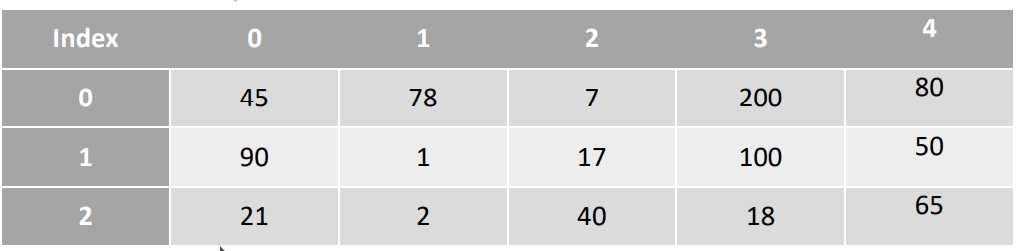
\includegraphics[width=.8\textwidth]{./images/2d-array.png}
                \end{figure}
                
                Based on data above, create a program to search data in 2d array, which the data to be searched is defined by user input (using sequential search).

                We can iterate through the 2d array be the row and columns. It will turn our loop from doing \texttt{$O(n)$} into \texttt{$O(n^2)$} shown on the code below

                \begin{minted}[autogobble,fontsize=\small]{java}
                    public int[] findInMatrix(int search, int[][] matrix) {
                        for (int i = 0; i < matrix.length; i++) {
                            for (int j = 0; j < matrix[i].length; j++) {
                                if (matrix[i][j] == search) return new int[]{i, j};
                            }
                        }
                        return null;
                    }
                \end{minted}

                We return \texttt{null} if it's not found and return a tuple of the \texttt{[row, column]} position if it's found
            }
        \end{itemize}
    }
    \pagebreak
    \item {
        There is 1D array as follows:
        
        \begin{figure}[h]
            \centering
            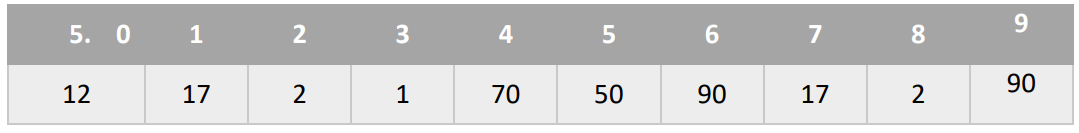
\includegraphics[width=.8\textwidth]{./images/1d-array.png}
        \end{figure}

        Create a program to sort the array, search \& display the biggest value, and print the amount of biggest value available alongside with its position.

        \begin{minted}[autogobble,fontsize=\footnotesize]{java}
            public class SingleDimensionArray {
                private static void displayData(int[] data) {
                    for (int i = 0; i < data.length; i++) {
                        System.out.printf("%s ", data[i]);
                    }
                    System.out.println();
                }

                private static void displayLargestValue(int[] data) {
                    int[] sortedData = sortAscending(data);
                    int[] largestValue = findLargestValue(sortedData);
                    System.out.println("Largest value position\t: " + largestValue[0]);
                    System.out.println("Largest value\t\t\t: " + largestValue[1]);
                }

                // returns a tuple of index and value
                private static int[] findLargestValue(int[] data) {
                    int largestPosition = 0;
                    int largest = data[largestPosition];
                    for (int i = 1; i < data.length; i++) {
                        if (data[i] > largest) {
                            largestPosition = i;
                            largest = data[largestPosition];
                        }
                    }
                    return new int[]{largestPosition, largest};
                }

                private static int[] sortAscending(int[] data) {
                    // uses insertion sort
                    for (int i = 1; i < data.length; i++) {
                        int tmp = data[i];
                        int j = i - 1;
                        while (j >= 0 && data[j] > tmp) {
                            data[j + 1] = data[j];
                            j--;
                        }
                        data[j + 1] = tmp;
                    }
                    return data;
                }

                private static int[] sortDescending(int[] data) {
                    // uses insertion sort
                    for (int i = 1; i < data.length; i++) {
                        int tmp = data[i];
                        int j = i - 1;
                        while (j >= 0 && data[j] < tmp) {
                            data[j + 1] = data[j];
                            j--;
                        }
                        data[j + 1] = tmp;
                    }
                    return data;
                }

                public static void main(String[] args) {
                    int[] data = {5, 7, 4, 32, 6, 7, 89, 56, 3, 5, 7, 78, 3};
                    System.out.println("Unsorted data: ");
                    displayData(data);

                    System.out.println("Sorted data (asc):");
                    int[] sortedDataAscending = sortAscending(data);
                    displayData(sortedDataAscending);

                    System.out.println("Sorted data (desc):");
                    int[] sortedDataDescending = sortDescending(data);
                    displayData(sortedDataDescending);

                    displayLargestValue(data);
                }
            }
        \end{minted}

        \begin{figure}[h]
            \centering
            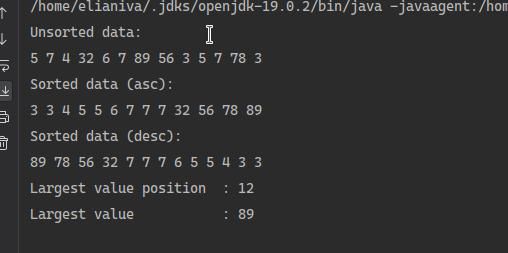
\includegraphics[width=.8\textwidth]{./images/1d-output.png}
        \end{figure}
    }
\end{enumerate}

\end{document}

